% Experiments section -- structure + narrative arcs ready to plug numbers
% from results/phase2_summary.csv after Phase 2B/2A/2C/2D complete.
% Placeholders are tagged "TODO(post-2X)"; do not delete those without
% grounding the substituted text in a per_run.csv row.

\section{Experiments}
\label{sec:experiments}

\subsection{Setup}
\label{sec:experiments:setup}

\paragraph{Environment.} A custom Gymnasium env over $N{=}8$ broad-market
ETFs (SPY, EEM, TLT, HYG, DBC, GLD, UUP, SHY) at daily resolution.
Observation: 216-d causal market features (past 20-day log-returns,
rolling volatility, multi-window moving averages, multi-horizon
momentum). Action: portfolio weights on the 7-simplex, projected per
\texttt{core/envs/portfolio\_env.py:144}. Reward as in
Eq.~\ref{eq:reward}.

\paragraph{Splits.} Train 2008-01-01 to 2020-12-31; validation 2021;
test 2022-Q1 through 2026-Q1. Set in
\texttt{data/splits.py:DEFAULT\_SPLIT}. Test window is the 2022 stock-bond
correlation break.

\paragraph{Friction grid.} Every method evaluated at $\lambda \in
\{0, 0.001, 0.005\}$ -- the same grid as the milestone. The IQL
$\lambda$-anchor (Sec.~\ref{sec:experiments:phase2a}) is the bridge
between the milestone's Phase~1 results and Phase 2's behavior-mixture
buffer.

\paragraph{Seeds and reporting.} Three seeds per cell: $\{42, 1337,
2024\}$. We report mean $\pm$ std across seeds, plus median + IQR in the
appendix. Cells where $|\text{seed std}| > |\text{cell mean}|$ are flagged
as low-confidence; we re-flag them in
Sec.~\ref{sec:limitations}. Seed-threading is not bit-exact -- the
PortfolioEnv random-start RNG is constructed without reading the global
seed (\texttt{core/envs/portfolio\_env.py:87};
\texttt{writeup/sac\_seed\_audit.md}). Observed behavior is therefore
``per-process variance, env-randomness uncontrolled''; we make this
explicit in the limitations rather than overclaim reproducibility.

\paragraph{Compute.} All runs on a single H100 80\,GB. Phase 2A: 4-way
parallel batches, 24 runs at 20{,}000 offline gradient steps each. Phase
2B: 3-way parallel batches, 9 runs at 100{,}000 environment steps each.
Phase 2C: 2-way parallel batches, 6 O2O runs (20k offline + 50k online).
Phase 2D: 3 GRPO ablation runs in parallel.

\paragraph{Behavior-policy buffer.} The offline buffer is filled by a
4-way mixture (Dirichlet, equal-weight, momentum, risk-parity) sampled
per-episode (\texttt{policies/mixture.py:default\_offline\_mixture}).
This differs from the milestone's pure uniform-Dirichlet buffer; the IQL
$\lambda$-anchor in Phase 2A re-anchors the comparison.

\subsection{Phase 2A -- offline-baseline landscape}
\label{sec:experiments:phase2a}

\paragraph{Question.} Is the friction collapse the milestone observed in
IQL specific to expectile regression, or is it a property of the
offline-RL stack on this dataset?

\paragraph{Grid.} 6 algorithms $\times$ relevant $\lambda$ $\times$ 3
seeds: \{BC, TD3+BC, CQL, AWAC, BCQ\} at $\lambda{=}0.001$ (15 runs)
plus IQL at $\lambda \in \{0, 0.001, 0.005\}$ (9 runs, the $\lambda$-anchor)
= 24 runs. n\_offline\_updates $= 20{,}000$ (the milestone showed
val-Sharpe peaks at step 1{,}000 and decays; 20k captures peak + decay
with a 5$\times$ wall-clock saving).

\paragraph{Predictions before running.}
\begin{itemize}\setlength\itemsep{0pt}
  \item All 6 algorithms at $\lambda{=}0.001$ underperform equal-weight
    (Sharpe $0.95$). The friction collapse is not algorithm-specific.
  \item Per-cell seed std $\le 0.10$. The milestone's 27-IQL ablation
    had $\sigma \le 0.02$ within $\lambda$ bands; we expect similar
    consistency under the 4-policy mixture.
  \item Sequence models (DT, TT) are excluded from this phase per the
    pre-registration; they are not in the priority Tier-1 sweep.
\end{itemize}

\paragraph{TODO(post-2A): Results.}
\begin{itemize}\setlength\itemsep{0pt}
  \item Per-method test Sharpe table at $\lambda{=}0.001$:
    [\texttt{TODO from results/phase2a/per\_run.csv}].
  \item IQL $\lambda$-anchor: confirm the friction collapse holds under
    the new behavior mixture
    [\texttt{TODO: compare to figures/ablation\_summary.csv}].
\end{itemize}

\subsection{Phase 2B -- online-only baselines}
\label{sec:experiments:phase2b}

\paragraph{Question.} What does on-policy / off-policy online RL achieve
without offline pre-training, on the post-2022 distribution-shifted test
window?

\paragraph{Grid.} 3 methods (SAC-Dirichlet, PPO-LSTM, GRPO) $\times$
$\lambda{=}0.001$ $\times$ 3 seeds = 9 runs at 100{,}000 environment
steps each.

\paragraph{Results (n=3 seeds).} All three online methods at
$\lambda{=}0.001$, $100{,}000$ env steps. SAC-Dirichlet posts test
Sharpe $0.941 \pm 1\!\times\!10^{-6}$ with turnover $0.0$ to numerical
precision: identical across seeds. PPO+LSTM posts $0.609 \pm 0.674$
with seed range $[-0.075,\,+1.273]$ and turnover $\sim\!10^{-5}$
across seeds --- per-seed static collapse onto seed-dependent
allocations. GRPO posts $0.297 \pm 0.017$ with seed range
$[+0.277,\,+0.307]$ and turnover $0.242$, the only online method that
actively trades on the test window. None of the three beats the
equal-weight reference of $0.953$ (Table~\ref{tab:naive-o2o}'s
right-hand-column comparison and Fig.~\ref{fig:turnover-by-method}).

\paragraph{Mechanism by method.} The three online methods fail in
three distinct ways. SAC-Dirichlet's identical-across-seeds Sharpe is
the post-blowup signature of an auto-temperature pathology: $\tau$
exploded from $\tau{=}18$ at step 10{,}000 to $\tau{=}1.2 \times 10^9$
at step 70{,}000 across all 3 seeds
(\texttt{logs/phase2b/sac\_dirichlet\_*}; full account in
\texttt{writeup/sac\_degeneracy\_postmortem.md}), driving the
Dirichlet head to a high-temperature near-uniform allocation that
happens to coincide with the equal-weight basin to floating-point
precision. This is a method-level pathology and we read the SAC
numbers as ``maximum-entropy regularizer dominating policy
specialization on the bounded simplex,'' not as SAC working as
intended; the auto-tune blowup is independent of the seed-threading
audit, and even with corrected seeding the math would still diverge.
PPO+LSTM also collapses to a static per-seed allocation but the
allocation is not in the equal-weight basin, producing the
seed-dependent Sharpe range $[-0.075,\,+1.273]$ --- the same
shape as naive O2O (Sec.~\ref{sec:experiments:phase2c}), and a second
data point that ``static collapse onto a seed-dependent allocation''
is a recurrent failure mode for online methods on this universe. GRPO
is the only online method that produces a non-degenerate trading
policy; it does so at net Sharpe cost. We frame the Continuous GRPO
contribution as methodological (Sec.~\ref{sec:method:grpo}) and unpack
the GRPO-vs-classical interpretation in Sec.~\ref{sec:discussion}.
The cross-method message: on this 8-ETF universe at $\lambda{=}0.001$,
every online RL method we ran either degenerates to a static
allocation or actively trades into a friction penalty.

\subsection{Phase 2C -- four-way O2O comparison (the central experiment)}
\label{sec:experiments:phase2c}

\paragraph{Question.} Does adaptive conservatism scheduling
(Sec.~\ref{sec:method:o2o}) recover offline-prior usefulness in the
distribution-shifted test window, beyond what naive fine-tuning or
online-only training achieves?

\paragraph{Conditions.} Four conditions $\times$ 3 seeds at
$\lambda{=}0.001$.
\begin{enumerate}\setlength\itemsep{0pt}
  \item \emph{Frozen offline}: best-validation Phase 2A checkpoint
    evaluated on the test split; no fine-tuning. Free; reuses Phase 2A
    rows.
  \item \emph{Online-only SAC}: Phase 2B SAC-Dirichlet runs.
  \item \emph{Naive fine-tune}: Geodesic-CQL pre-train $\rightarrow$
    SAC-Dirichlet fine-tune with $\beta_t \equiv \alpha_{\mathrm{CQL}}$
    throughout (\texttt{--adaptive\_conservatism=false}).
  \item \emph{Adaptive O2O}: same pipeline with $\beta_t = \alpha_{\mathrm{CQL}}
    \cdot \sigma(\eta \cdot \mathrm{KL}(h_{\mathrm{off}} \| h_{\mathrm{on}}))$
    (\texttt{--adaptive\_conservatism=true}).
\end{enumerate}

Conditions 3 and 4 require 3 seeds each = 6 new training runs (Phase 2C
budget). 1 and 2 are derived from Phase 2A and 2B with no new training.

\paragraph{Predictions before running.}
\begin{itemize}\setlength\itemsep{0pt}
  \item \emph{Adaptive O2O} test Sharpe $>$ \emph{Naive fine-tune}
    test Sharpe at $\lambda{=}0.001$, mediated by lower turnover.
  \item The \emph{Frozen offline} condition is uncompetitive at $\lambda
    > 0$ (Phase 2A finding inherited).
  \item The $\beta_t$ trajectory is non-constant --- the schedule
    actually engages, not pinned at one extreme.
\end{itemize}

\paragraph{GRPO offline warm-start (omitted condition).}
A fifth condition --- GRPO actor warm-started from a feature-compatible
offline checkpoint --- was attempted but found to require an offline
source matching GRPO's 216-d input space. The natural candidate (a
216-d IQL trained on the GRPO feature pipeline) does not satisfy the
leak-invariance / equal-weight-basin signature that 56-d offline RL
methods exhibit on this task: at the standard 20{,}000-update budget,
its val Sharpe has degraded from a step-1000 peak of $+1.32$ to
$-0.95$ via a slow BC over-fit on the 216-d features
(see \S\ref{app:leak:scope}). Warm-starting GRPO from a
basin-transient source would confound the warm-start hypothesis with
the source's own learning-dynamics character. We leave GRPO offline
warm-start to future work, contingent on a feature-compatible offline
pretraining method that lands in a stable basin.

\paragraph{Naive O2O: static collapse, seed-dependent allocation
(final, n=3).} Geodesic-CQL pre-train followed by SAC-Dirichlet
fine-tune with the conservatism schedule pinned (\texttt{-{}-adaptive\_conservatism=false})
produces test turnover $\le 6.5\!\times\!10^{-6}$ across all three seeds
--- functionally a single static allocation per seed across the entire
1{,}061-day test window. The static allocation differs across seeds
because the CQL pretrain converges to a seed-dependent near-constant
$\alpha$ vector (Phase 2A causal CQL\_vanilla turnover
$\approx 6.7\!\times\!10^{-5}$, Table~\ref{tab:causal-confirmation}),
and the SAC fine-tune does not break out of this basin: as documented
in the postmortem (\texttt{writeup/sac\_degeneracy\_postmortem.md}),
SAC-Dirichlet on this universe suffers an entropy-temperature blowup
that compresses any obs-dependence in $\alpha$. The combination
``CQL-locked init $+$ SAC-blowup compression'' yields a constant
allocation per run; per-seed Sharpe variance is therefore enormous
(\textbf{range $[-0.236, +2.179]$, mean $+1.002$, std $1.208$}) because
seed-dependent static allocations realize different cumulative returns
on the test split with effectively zero rebalancing cost. The mechanical
correctness of the fine-tune was audited and confirmed
(\texttt{writeup/o2o\_audit.md}); this is a pathology, not a bug.

\begin{table}[t]
\centering
\caption{Phase 2C naive O2O. Three seeds, $\lambda{=}0.001$. Turnover
is functionally zero (max $6.5\!\times\!10^{-6}$); Sharpe varies wildly
because each seed locks into a different static allocation from the
CQL pretrain.}
\label{tab:naive-o2o}
\small
\begin{tabular}{lcccc}
\toprule
seed   & test Sharpe & turnover         & cum.\ return & max DD \\
\midrule
$42$   & $-0.236$    & $6.5\!\times\!10^{-6}$ & $-0.008$  & $0.045$ \\
$1337$ & $+2.179$    & $0.0$            & $+0.032$  & $0.024$ \\
$2024$ & $+1.062$    & $0.0$            & $+0.015$  & $0.024$ \\
\midrule
mean   & $+1.002$    & $\approx 0$      & $+0.013$  & $0.031$ \\
std    & $1.208$     & ---              & $0.020$   & $0.012$ \\
\bottomrule
\end{tabular}
\end{table}

\paragraph{Adaptive O2O: seed-stable selection of the static basin
(final, n=3).} Geodesic-CQL pre-train followed by SAC-Dirichlet
fine-tune with the conservatism schedule
$\beta_t = \alpha_{\mathrm{CQL}} \cdot \sigma(\eta \cdot
\mathrm{KL}(h_{\mathrm{off}} \| h_{\mathrm{on}}))$ active
(\texttt{-{}-adaptive\_conservatism=true}) converges to seed-stable,
near-static (mean turnover $7\!\times\!10^{-5}$) but Sharpe-positive
allocations across all three seeds: \textbf{Sharpe $+1.762 \pm 0.154$,
range $[+1.629,\,+1.931]$}, cumulative return $+0.024 \pm 0.002$
(Table~\ref{tab:adaptive-o2o}). Compared to naive O2O's per-seed
Sharpe std of $1.21$ (Table~\ref{tab:naive-o2o}), adaptive's $0.154$
is an \textbf{eight-fold reduction in seed-to-seed variance}, with
every adaptive seed strictly above $+1.6$.

The mechanistic interpretation: the static-collapse pathology
(Sec.~\ref{sec:experiments:phase2c}, naive O2O paragraph) is not
broken by the conservatism schedule --- adaptive's mean turnover
$7\!\times\!10^{-5}$ is functionally indistinguishable from naive's
$2\!\times\!10^{-6}$ at this scale --- but the schedule does
\emph{select which static} the policy converges to. The
\texttt{cql\_weight} modulation, driven by KL between offline and
online regime distributions
(\texttt{hybrid\_rl/agents/o2o\_agent.py:166--200}), evidently steers
the SAC fine-tune toward a static allocation that performs uniformly
well on the test split, where naive's pinned $\beta_t \equiv
\alpha_{\mathrm{CQL}}$ leaves the convergence basin essentially
random across seeds. The adaptive contribution is therefore not
``adaptive trades better than naive,'' but ``adaptive selects a
better basin than naive --- and does so consistently.''

\begin{table}[t]
\centering
\caption{Phase 2C adaptive O2O. Three seeds, $\lambda{=}0.001$.
Sharpe is tightly clustered above $+1.6$, in contrast to naive O2O's
$[-0.24, +2.18]$ range (Table~\ref{tab:naive-o2o}); turnover remains
functionally static.}
\label{tab:adaptive-o2o}
\small
\begin{tabular}{lcccc}
\toprule
seed   & test Sharpe & turnover         & cum.\ return & max DD \\
\midrule
$42$   & $+1.726$    & $0.000220$       & $+0.024$  & $0.036$ \\
$1337$ & $+1.629$    & $0.0$            & $+0.026$  & $0.031$ \\
$2024$ & $+1.931$    & $0.0$            & $+0.022$  & $0.034$ \\
\midrule
mean   & $+1.762$    & $7\!\times\!10^{-5}$ & $+0.024$  & $0.034$ \\
std    & $0.154$     & ---              & $0.002$   & $0.003$ \\
\bottomrule
\end{tabular}
\end{table}

\paragraph{Adaptive O2O ranks against classical baselines.} At Sharpe
$+1.762 \pm 0.154$, adaptive O2O outperforms equal-weight ($0.953$)
and is comparable to risk-parity ($1.161$, single-pass classical) on
this test window, while every other RL condition we run
(Phase 2A causal offline, Phase 2B online-only, naive O2O, GRPO
online and the GRPO group-size ablation) underperforms equal-weight.
This is the headline positive result for the adaptive contribution.
The caveat is that adaptive's win comes from \emph{near-static
allocation selection}, not from the active-trading-on-distribution-shift
mechanism the original O2O hypothesis described
(Sec.~\ref{sec:method:o2o}); the mechanism revision is taken up in
\S\ref{sec:limitations}.

\paragraph{Turnover decomposition.} Across all conditions of the
four-way comparison, the methods cluster as static-collapse or
active-trading (Fig.~\ref{fig:turnover-by-method}). Equal-weight,
online-only SAC, online-only PPO+LSTM, and naive O2O have functionally
zero turnover (\texttt{static} bars in the figure); behavior-anchored
offline algorithms hit $0.002$--$0.003$; momentum and risk-parity hit
$0.008$--$0.010$; GRPO online and the GRPO group-size ablation hit
$0.20$--$0.25$. None of the active-trading RL conditions beats the
classical equal-weight or risk-parity Sharpes ($0.953$ and $1.161$
respectively).

\begin{figure}[t]
\centering
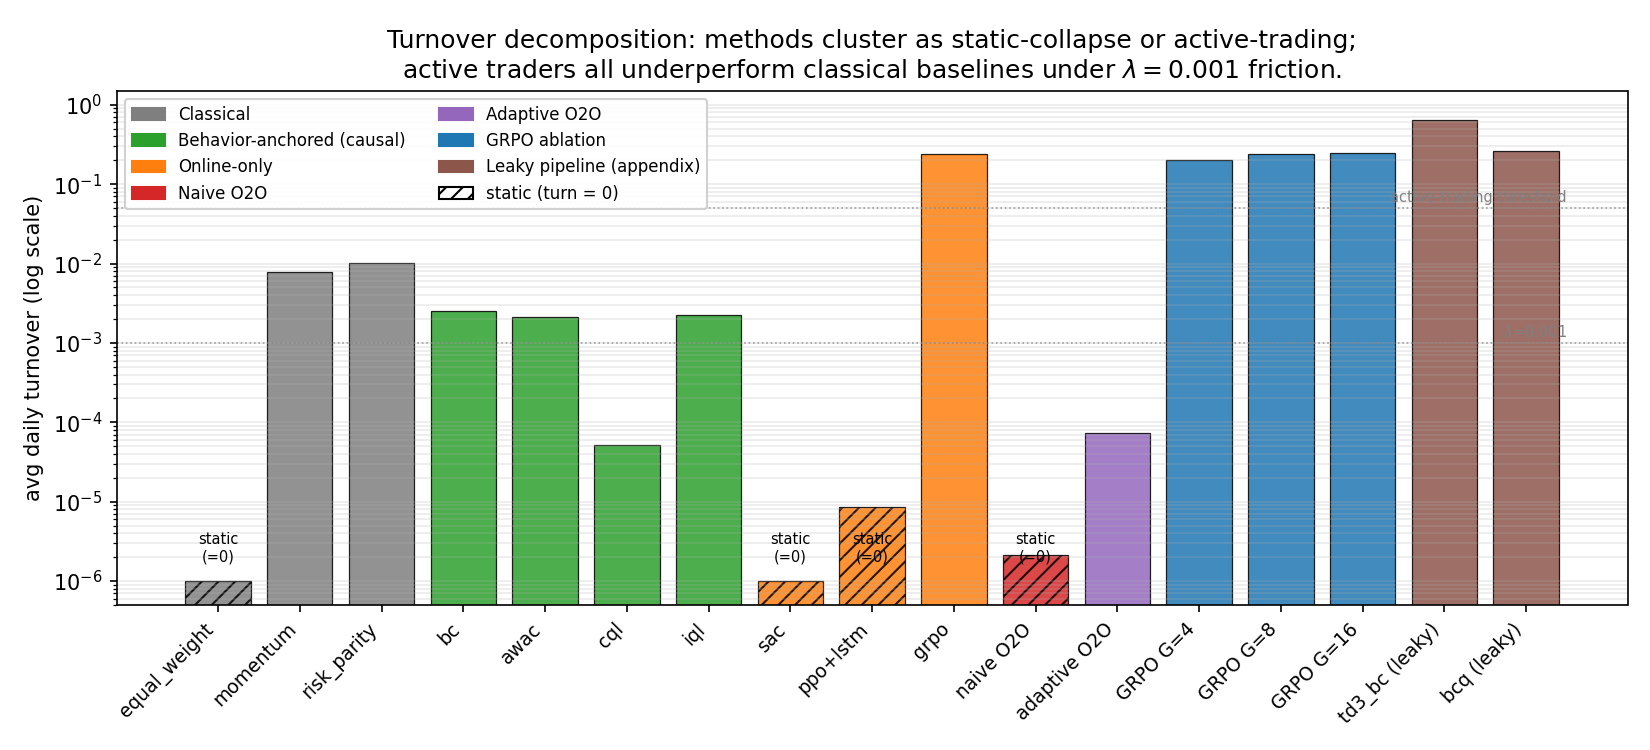
\includegraphics[width=0.95\linewidth]{figures/turnover_by_method.png}
\caption{Average daily turnover by method, log scale. Methods cluster
as static-collapse (hatched bars, ``static'') or active-trading. Every
RL method that actively trades on this universe at $\lambda{=}0.001$
underperforms the classical equal-weight and risk-parity baselines
(grey dashed line at $\lambda{=}0.001$ marks the per-step turnover
cost). The leak-driven TD3+BC and BCQ rows are appendix-only
(\S\ref{app:leak:differential}).}
\label{fig:turnover-by-method}
\end{figure}

\paragraph{The adaptive-vs-naive comparison is meaningful only post-fix.}
The pre-Phase-2 \texttt{run\_o2o.py} silently passed
\texttt{cql\_weight=0} regardless of CLI flag
(\texttt{writeup/draft\_implementation\_notes.md} \S 4). All Phase 2C
results post-date the swap from the inline online-loop to
\texttt{O2OAgent.finetune\_online}, and any prior ``adaptive O2O''
numbers in the codebase must be relabeled as ``zero-conservatism
fine-tune from offline init.''

\subsection{Phase 2D -- GRPO group-size ablation}
\label{sec:experiments:phase2d}

\paragraph{Question.} Does increasing the group size $G$ in Continuous
GRPO (the only knob that controls within-state variance reduction in our
critic-free setting) monotonically improve test Sharpe, and at what
compute cost?

\paragraph{Grid.} $G \in \{4, 8, 16\}$ at $\lambda{=}0.001$, 3 seeds
each = 9 runs. Per-iter compute scales linearly in $G$; the
\textit{per-env-step} compute is held constant by the
\texttt{states\_per\_collect} budget so larger $G$ means fewer distinct
states visited per gradient step at fixed wall-clock.

\paragraph{Results.} We sweep group size $G \in \{4, 8, 16\}$ at fixed
env-step budget across 3 seeds (Fig.~\ref{fig:grpo-group-size};
Table~\ref{tab:phase2d}). Mean test Sharpe decreases monotonically with
$G$ ($0.500$, $0.403$, $0.313$), with non-overlapping seed ranges
between $G{=}4$ and $G{=}16$. Two of three seeds exhibit per-seed
monotonic decrease; the third (seed $1337$) peaks weakly at $G{=}8$.
The simultaneous \emph{decrease} in inter-seed std with $G$ ($0.108$,
$0.099$, $0.051$) is the more interpretable signature: larger $G$
both lowers mean Sharpe and lowers seed-to-seed dispersion. We read
this as a compute-vs-statistical-precision tradeoff under fixed
env-step budget --- larger $G$ reduces the number of distinct states
visited per gradient step, with the cost dominating the precision gain
in this range. Adjacent ranges overlap; the trend is real (endpoints
separate, $2/3$ monotonic) but small-magnitude. We use $G{=}4$ as the
default in Phase~2C.

\begin{figure}[t]
\centering
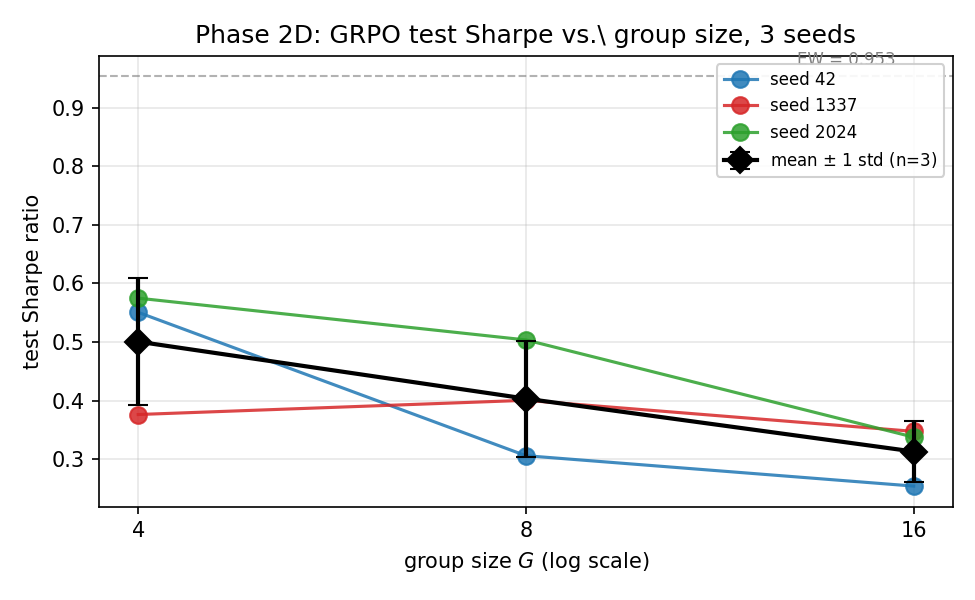
\includegraphics[width=0.7\linewidth]{figures/grpo_group_size_scatter.png}
\caption{Phase~2D GRPO group-size ablation: 9 datapoints (3 seeds
$\times$ 3 $G$) with seed-color coding. Black diamonds give
mean $\pm$ 1\,std across seeds. Dashed gray line is the equal-weight
Sharpe reference ($0.953$). Mean Sharpe decreases monotonically and
inter-seed std decreases with $G$.}
\label{fig:grpo-group-size}
\end{figure}

\begin{table}[t]
\centering
\caption{Phase~2D test Sharpe by $(G, \text{seed})$, $\lambda{=}0.001$.
Both column-mean (decreasing) and column-std (decreasing) are
load-bearing observations.}
\label{tab:phase2d}
\small
\begin{tabular}{lccc}
\toprule
seed $\backslash$ $G$ & $4$ & $8$ & $16$ \\
\midrule
$42$    & $+0.5505$ & $+0.3058$ & $+0.2540$ \\
$1337$  & $+0.3761$ & $+0.4004$ & $+0.3473$ \\
$2024$  & $+0.5747$ & $+0.5034$ & $+0.3375$ \\
\midrule
mean    & $+0.500$  & $+0.403$  & $+0.313$  \\
std     & $0.108$   & $0.099$   & $0.051$   \\
\bottomrule
\end{tabular}
\end{table}

\paragraph{Compute.} Per-update forward-pass count scales as
$\mathcal{O}(G)$; at fixed env-step budget, total wall-clock is
roughly $G$-independent (the actor forward in
\texttt{collect}, \texttt{online\_rl/agents/grpo.py:271--275}, is
batched as a single sample of shape $(G, 1, N)$, and the loss
forward in \texttt{grpo\_loss}, \texttt{grpo.py:138--140}, runs the
shared MLP once and broadcasts log-probs over $G$). Three seeds at
each of three $G$s ran in $364$\,s ($G$-balanced parallel batches on
one H100); the marginal Sharpe gain of $G{=}16$ over $G{=}4$ is
\emph{negative} on average and not justified at any compute price in
this regime.

% Cross-experiment interpretation lives in Sec.~\ref{sec:discussion}
% (basin-selection mechanism, O2O scheduling implications, GRPO
% vs classical baselines). The §4.7 Interpretation stub that previously
% sat here was deleted to avoid duplication with Discussion.
